\documentclass[11pt, dvipsnames, handout]{beamer}
\newtoggle{full}
\settoggle{full}{true}

\newtoggle{covered}
\settoggle{covered}{false}

\newtoggle{presentable}
\settoggle{presentable}{false}

\newtoggle{dualscreen}
\settoggle{dualscreen}{false}

\usepackage{pgfplots}
%\pgfplotsset{compat = newest}

\usepackage{pgfpages}

\setbeamertemplate{note page}{\pagecolor{yellow!5}\vfill \insertnote \vfill}
\usepackage{collect}
\definecollection{notes}
\newcounter{notestaken}

\usepackage{xpatch}

\usepackage{ulem}

\usepackage[framemethod=tikz]{mdframed}

\usepackage{scalerel}
\usepackage{calc}

%\usepackage{enumitem}
\setlength\fboxsep{.2em}

\usepackage{graphicx} % Allows including images
\usepackage{booktabs} % Allows the use of \toprule, \midrule and \bottomrule in tables

\xpatchcmd{\itemize}
  {\def\makelabel}
  {\setlength{\itemsep}{0.65 em}\def\makelabel}
  {}
  {}


\xpatchcmd{\beamer@enum@}
  {\def\makelabel}
  {\setlength{\itemsep}{0.65 em}\def\makelabel}
  {}
  {}


%\makeatletter
%\renewcommand{\itemize}[1][]{%
%  \beamer@ifempty{#1}{}{\def\beamer@defaultospec{#1}}%
%  \ifnum \@itemdepth >2\relax\@toodeep\else
%    \advance\@itemdepth\@ne
%    \beamer@computepref\@itemdepth% sets \beameritemnestingprefix
%    \usebeamerfont{itemize/enumerate \beameritemnestingprefix body}%
%    \usebeamercolor[fg]{itemize/enumerate \beameritemnestingprefix body}%
%    \usebeamertemplate{itemize/enumerate \beameritemnestingprefix body begin}%
%    \list
%      {\usebeamertemplate{itemize \beameritemnestingprefix item}}
%      {%
%        \setlength\topsep{1em}%NEW
%        \setlength\partopsep{1em}%NEW
%        \setlength\itemsep{1em}%NEW
%        \def\makelabel##1{%
%          {%
%            \hss\llap{{%
%                \usebeamerfont*{itemize \beameritemnestingprefix item}%
%                \usebeamercolor[fg]{itemize \beameritemnestingprefix item}##1}}%
%          }%
%        }%
%      }
%  \fi%
%  \beamer@cramped%
%  \raggedright%
%  \beamer@firstlineitemizeunskip%
%}
%
%
%
%
%
%\makeatother

%\setlist[beamer@enum@]{topsep=1 em}
%\let\origcheckmark\checkmark %screw you dingbat
%\let\checkmark\undefined %screw you dingbat
%\usepackage{dingbat} 
%\let\checkmark\origcheckmark %screw you dingbat






%\usepackage{fontawesome}

\usepackage{mathtools}
\usepackage{etoolbox, calculator}

\usepackage{xcolor}
\usepackage{tikz}
\usetikzlibrary{arrows.meta}
\usetikzlibrary{calc}
\usepackage[nomessages]{fp}
\usepackage{transparent}
\usepackage{accsupp}
%\usepackage{color, xcolor}

%colorblind-friendly palette
%\definecolor{dblue}{RGB}{51,34,136}
\definecolor{lblue}{RGB}{136,204,238}
%\definecolor{green}{RGB}{17,119,51}
\definecolor{tan}{RGB}{221,204,119}
%\definecolor{mauve}{RGB}{204,102,119}

\usepackage{tcolorbox}



\usepackage{xifthen}
\usepackage{nicefrac}
\usepackage{amsmath}
\usepackage{amsthm}
\usepackage{amssymb}
\theoremstyle{definition}
\newtheorem*{define}{Definition}
\newtheorem*{recall}{Recall}


\DeclareMathOperator{\tr}{tr}

\usepackage{multicol}
%\setlength{\columnsep}{1cm}

\usepackage{tablists, amsmath,vwcol, cancel, polynom}
\usetikzlibrary{shapes, patterns, decorations.shapes}
%\usepackage{tikzpeople}
\tikzstyle{vertex}=[shape=circle, minimum size=2mm, inner sep=0, fill]
\tikzstyle{opendot}=[shape=circle, minimum size=2mm, inner sep=0, fill=white, draw]

% common math quick commands
\newcommand{\nicedd}[2]{\nicefrac{\text{d}#1}{\text{d}#2}}
\newcommand{\dd}[2]{\dfrac{\text{d}#1}{\text{d}#2}}
\newcommand{\pd}[2]{\dfrac{\partial #1}{\partial#2}}
\renewcommand{\d}[1]{\text{d}#1}
\newcommand{\ddn}[3]{\dfrac{\text{d}^{#3}#1}{\text{d}#2^{#3}}}
\newcommand{\pdn}[3]{\dfrac{\partial^{#3}#1}{\partial#2^{#3}}}
\newcommand{\p}[0]{^{\prime}}
\newcommand{\pp}[0]{^{\prime\prime}}
\newcommand{\op}[2][\text{L}]{#1 \left[ #2 \right]}

\newcommand{\lap}[1]{\mathcal{L}\left\{#1\right\}}
\newcommand{\lapinv}[1]{\mathcal{L}^{-1}\left\{#1\right\}}
\newcommand{\lapint}[1]{\int_0^\infty e^{-st}#1dt}
\newcommand{\evalat}[2]{\Big|_{#1}^{#2}}

\newcommand{\paren}[1]{ \left( #1 \right)}

\newcommand{\haxis}[4][\normcolor]{\draw[#1, <->] (-#2,0)--(#3,0) node[right]{$#4$}; }


\newcommand{\axis}[4]{\draw[\normcolor, <->] (-#1,0)--(#2,0) 
node[right]{$x$};
\draw[help lines, <->] (0,-#3)--(0,#4) node[above]{$y$};}

\newcommand{\laxis}[6]{\draw[<->] (-#1,0)--(#2,0) 
node[right]{$#5$};
\draw[ <->] (0,-#3)--(0,#4) node[above]{$#6$};}
\newcommand{\xcoord}[2]{
	\draw (#1,.2)--(#1,-.2) node[below]{$#2$};}
\newcommand{\textnode}[3]{
	\draw (#1,#2) node[below]{$#3$};}
	
\newcommand{\nxcoord}[2]{
	\draw (#1,-.2)--(#1,.2) node[above]{$#2$};}
\newcommand{\ycoord}[2]{
	\draw (.2,#1)--(-.2,#1) node[left]{$#2$};}
\newcommand{\nycoord}[2]{
	\draw (-.2,#1)--(.2,#1) node[right]{$#2$};}
\newcommand{\dlim}{\displaystyle\lim}
\newcommand{\dlimx}[1]{\displaystyle\lim_{x \rightarrow #1}}
\newcommand{\stickfig}[2]{
	\draw (#1,#2) arc(-90:270:2mm);
	\draw (#1,#2)--(#1,#2-.5) (#1-.25,#2-.75)--(#1,#2-.5)--(#1+.25,#2-.75) (#1-.2,#2-.2)--(#1+.2,#2-.2);}	

%\newcounter{example}
%\setcounter{example}{1}
%\newcounter{preFrameExample}
%\AtBeginEnvironment{frame}{\setcounter{preFrameExample}{\value{example}}}
%\newcommand{\ex}[1]{
%	 \setcounter{example}{\value{preFrameExample}}
%	 \textcolor{green}{\small\fbox{Example \arabic{example}: #1}}\\[8pt]
%	\stepcounter{example}}
%\newcommand{\exans}[1]{
%	\SUBTRACT{\value{preFrameExample}}{1}{\n}
%	 \textcolor{green}{\small\fbox{Solution \n: #1}}\\[8pt]}
\mode<presentation> {

% The Beamer class comes with a number of default slide themes
% which change the colors and layouts of slides. Below this is a list
% of all the themes, uncomment each in turn to see what they look like.


\usetheme{CambridgeUS}
\usecolortheme[named=black]{structure}


\newcommand{\studentcolor}[0]{ForestGreen}
\newcommand{\normcolor}[0]{NavyBlue}
\newcommand{\alertcolor}{Red}

\setbeamercolor{normal text}{fg=\normcolor}
\setbeamercolor{frametitle}{fg=\normcolor}
\setbeamercolor{section in head/foot}{fg=Black, bg=Gray!20}
\setbeamercolor{subsection in head/foot}{fg=Green!70!Black, bg=Gray!10}
\setbeamercolor{alerted text}{fg=\alertcolor}
\setbeamerfont{alerted text}{series=\bf}
\setbeamertemplate{enumerate items}[default]
\setbeamercolor{enumerate item}{fg=\normcolor}

\setbeamertemplate{footline} % To remove the footer line in all slides uncomment this line
%\setbeamertemplate{footline}[page number] % To replace the footer line in all slides with a simple slide count uncomment this line

\setbeamertemplate{navigation symbols}{} % To remove the navigation symbols from the bottom of all slides uncomment this line
}

\newcommand{\alertbox}[1]{\tcbox[on line, colframe=\alertcolor, colback=White, left=2pt,right=2pt,top=2pt,bottom=2pt]{\usebeamercolor*{normal text}#1}}


\newcommand{\startstu}{\setbeamercolor{normal text}{fg=\studentcolor}\usebeamercolor*{normal text}\setbeamercolor{enumerate item}{fg=\studentcolor}\usebeamercolor*{enumerate item}}
\newcommand{\stopstu}{\setbeamercolor{normal text}{fg=\normcolor}\usebeamercolor*{normal text}\setbeamercolor{enumerate item}{fg=\normcolor}\usebeamercolor*{enumerate item}}

\newcommand{\takenote}[1]{ \begin{collect}{notes}{}{}{}{}  #1  \end{collect}  \addtocounter{notestaken}{1}} %\ifthenelse{\value{notestaken}>0}{\hrulefill\\}{}

\makeatletter
\newcommand{\cover}{\alt{\beamer@makecovered}{\beamer@fakeinvisible}}
\newcommand{\ucover}[1]{\iftoggle{full}{}{\beamer@endcovered}\stopstu#1\startstu\iftoggle{full}{}{\beamer@startcovered}}
\makeatother

\newcommand{\skippause}{ \addtocounter{beamerpauses}{-1}}
\newcommand{\blockpres}{ \skippause \pause }

\newcommand{\studentify}[1]{\startstu #1  \stopstu }
\newcommand{\student}[1]{\iftoggle{full}{ \pause  \studentify{#1} }{\iftoggle{covered}{\studentify{#1}}{\cover{  #1 }}}}
\newcommand{\cstudent}[1]{\student{\begin{center} #1 \end{center}}}
\newcommand{\fullonly}[1]{\iftoggle{full}{ #1}{}}
\newcommand{\presentonly}[1]{\iftoggle{presentable}{ #1}{}}

\usepackage{xparse}
\usepackage{xifthen}

% shortcuts for commonly-used presentation elements
%\NewDocumentCommand{\slide}{o m}
% {\IfValueTF{#1}{\begin{frame}[t]{#1}}{\begin{frame}[t]} #2 \end{frame}}

\newtoggle{iscovered}

\newcommand{\slide}[2][]{%
%\setcounter{notestaken}{0}
\takenote{#2} 
%\ifthenelse{\equal{#1}{}}{\begin{frame}[t]}{\begin{frame}[t]{#1}} #2 \ifthenelse{\value{notestaken}>0}{ \note{\includecollection{notes}}}{} \end{frame}%
\ifthenelse{\equal{#1}{}}{\begin{frame}[t]}{\begin{frame}[t]{#1}} #2 \iftoggle{covered}{\settoggle{iscovered}{true}}{\settoggle{iscovered}{false}}  \note{ \iftoggle{iscovered}{}{\settoggle{covered}{true}} #2 \iftoggle{iscovered}{}{\settoggle{covered}{false}} } \end{frame}%
%\setcounter{notestaken}{0}
}
\newcommand{\defn}[2][]{%
 \setcounter{listcounter}{0}%
\ifthenelse{\equal{#1}{}}{\begin{block}{Definition}}{\begin{block}{#1 :}}%
 #2 \vspace{0.25em} \ifthenelse{\value{listcounter}>0}{\skippause}{} \pause \end{block}%
}



\newcommand{\arr}[2]{\begin{array}{#1}#2\end{array}}
\newcommand{\mat}[2]{\left[\arr{#1}{#2}\right]}
\newcommand{\carray}[1]{\arr{c}{#1}}
\newcommand{\larray}[1]{\arr{l}{#1}}
\newcommand{\rarray}[1]{\arr{r}{#1}}
\newcommand{\colvec}[1]{\mat{c}{#1}}

\newcommand{\itmz}[1]{\addtocounter{listcounter}{1} \begin{itemize}#1 \end{itemize} }
\newcommand{\subitem}[1]{\addtocounter{listcounter}{1} \begin{itemize} \item #1 \end{itemize}}
%
\newcommand{\enum}[1]{\addtocounter{listcounter}{1} \begin{enumerate} #1  \end{enumerate}  }


\newcommand{\algnlbl}[1]{\begin{align}#1  \end{align}} 
\newcommand{\algn}[1]{\begin{align*}#1  \end{align*}} 
\newcommand{\lgn}[1]{ \action<+->{#1} }
\newcommand{\slgn}[1]{\iftoggle{full}{\action<+->{ \startstu #1 \stopstu}}{ \cover{ #1 } } \takenote{$#1$}}

\newcommand{\chckmrk}{\alert{\checkmark}}

\usepackage{pifont}
\newcommand{\xmark}{\alert{\text{\large \ding{55}}}}

\newcommand{\return}[0]{\raisebox{.5ex}{\rotatebox[origin=c]{180}{$\Lsh$}}}
\usepackage{pbox}
%\newcommand{\ex}[1]{\rotatebox[origin=c]{10}{\uline{ex}}:$\;$\pbox[t][][b]{0.9\linewidth}{#1}}
\newcommand{\ex}[1]{\uline{ex}:$\;$\pbox[t][][t]{0.9\linewidth}{#1}}
\newcommand{\eg}[1]{e.g.,$\;$\pbox[t][][t]{0.9\linewidth}{#1}}
\newcommand{\tikzplot}[8][]{%
\begin{tikzpicture}

\begin{scope}[]%
\clip(-#2,-#4) rectangle (#3,#5);%
#8%
\end{scope}%
\laxis{#2}{#3}{#4}{#5}{#6}{#7}%
#1
\end{tikzpicture}%
}


\newcommand{\cancelslide}[1]{%
\begingroup%
\setbeamertemplate{background canvas}{%
\begin{tikzpicture}[remember picture,overlay]%
\draw[line width=2pt,red!60!black] %
  (current page.north west) -- (current page.south east);%
\draw[line width=2pt,red!60!black] %
  (current page.south west) -- (current page.north east);%
\end{tikzpicture}}%
#1%
\endgroup%
}
\renewcommand{\CancelColor}{\color{red}}
\newcommand{\twocols}[3][0.5]{\begin{columns}\begin{column}{#1\textwidth}#2\end{column}\hspace{1em}\vrule{}\hspace{1em}\begin{column}{#1\textwidth}#3\end{column}\end{columns}}

\newcommand{\twomini}[5][1]{\calculatespace \begin{minipage}[t]{\columnwidth}\begin{minipage}[][#1\contentheight][t]{#2\columnwidth}#4\end{minipage}\hfill\begin{minipage}[][#1\contentheight][t]{#3\columnwidth}#5\end{minipage}\end{minipage}}

\newcommand{\threemini}[7][1]{\calculatespace \begin{minipage}[t]{\columnwidth}\begin{minipage}[][#1\contentheight][t]{#2\columnwidth}#5\end{minipage}\hfill\begin{minipage}[][#1\contentheight][t]{#4\columnwidth}#6\end{minipage}\hfill\begin{minipage}[][#1\contentheight][t]{#3\columnwidth}#7\end{minipage}\end{minipage}}


\newcounter{listcounter}
\setcounter{listcounter}{0}



\newif\ifsidebartheme
\sidebarthemetrue

\newdimen\contentheight
\newdimen\contentwidth
\newdimen\contentleft
\newdimen\contentbottom
\makeatletter
\newcommand*{\calculatespace}{%
\contentheight=\paperheight%
\ifx\beamer@frametitle\@empty%
    \setbox\@tempboxa=\box\voidb@x%
  \else%
    \setbox\@tempboxa=\vbox{%
      \vbox{}%
      {\parskip0pt\usebeamertemplate***{frametitle}}%
    }%
    \ifsidebartheme%
      \advance\contentheight by-1em%
    \fi%
  \fi%
\advance\contentheight by-\ht\@tempboxa%
\advance\contentheight by-\dp\@tempboxa%
\advance\contentheight by-\beamer@frametopskip%
\ifbeamer@plainframe%
\contentbottom=0pt%
\else%
\advance\contentheight by-\headheight%
\advance\contentheight by\headdp%
\advance\contentheight by-\footheight%
\advance\contentheight by4pt%
\contentbottom=\footheight%
\advance\contentbottom by-4pt%
\fi%
\contentwidth=\paperwidth%
\ifbeamer@plainframe%
\contentleft=0pt%
\else%
\advance\contentwidth by-\beamer@rightsidebar%
\advance\contentwidth by-\beamer@leftsidebar\relax%
\contentleft=\beamer@leftsidebar%
\fi%
}
\makeatother


\usepackage{listings}

\iftoggle{dualscreen}{\setbeameroption{show notes on second screen=right}}{}
\begin{document}
\section{Lecture 3}
\subsection{Introduction}

\slide[Recall:]{
\vspace{-1em}
We saw how to use integration to solve the following first order ODEs\vfill
\[ y\p = f(t), \quad  y\p=f(y), \text{ and} \quad y'=g(y)f(t).\]\vfill
What happens if\enum{\item we cannot solve one of the integrals, or \item we get a more general ODE of the form $y'=f(y,t)$?}\vfill
\student{Exact analytical solutions are not always possible.\vfill \subitem{99.99\% of all the possible ODEs involve impossible integrals.}\vfill
Today we will build intuition around how to find approximate solutions.
}
}


\subsection{ Graphical intuition and the direction field}

\slide[Graphical intuition, whats does $y\p = f(y,t)$ mean?]{\vspace{-.5em}
\twomini[.58]{.4}{.59}{\vspace{-.5em}
\tikzplot{1}{3.25}{.5}{3.25}{t}{y(t)}{
\draw[thick, black] (0,3) .. controls (0,1) and (1,3) .. (3.5,-1);
\def\x0{1.6}
\def\y0{1.28}
\def\dx{.6}
\def\slope{-.77}
\def\spacer{.25}
\draw[ultra thick,->] (\x0-\dx,\y0-\dx*\slope) -- (\x0+\dx,\y0+\dx*\slope);
\node[vertex] at (\x0, \y0) {};
\draw[thick,|-|] (\x0-\dx,\y0+\dx*\slope-\spacer) -- (\x0+\dx,\y0+\dx*\slope-\spacer) node[midway, below]{$\Delta t$};
\draw[thick,|-|] (\x0-\dx-\spacer,\y0-\dx*\slope) -- (\x0-\dx-\spacer,\y0+\dx*\slope) node[midway, left]{$\Delta y$};
}


}
{

\[ \dd{y}{t} = f(y,t) \]

\student{
\vspace{.5em}
\algn{f(y,t) &= \text{slope of y(t) in the $(t,y)$-plane.}\\
&\approx\frac{\Delta y}{\Delta t}}



}
}
\uline{Slope Field Diagram:}\vfill
\student{ \enum{\item Draw an arrow with slope $f(y,t)$ for some points in the $(t,y)$-plane.\vfill
\item Stating from some initial condition(s), trace along with the arrows to get approximate solutions.} }
}

\presentonly{
\slide[Example: $y\p=2-y$, try different initial conditions]{
\twomini{.4}{.6}{

\resizebox{5.25cm}{7cm}{
\begin{tikzpicture}\hspace{-.5cm}
\begin{axis}[
    xmin = -0.5, xmax = 3.5,
    ymin = -1.5, ymax = 4.5,
    zmin = 0, zmax = 1,
    grid=minor,
    grid style={line width=.1pt},
    major grid style={line width=.2pt},
    minor tick num=1,
    xtick = {0,1,2,3},
    ytick = {-1,0,1,2,3,4},
    axis equal image,
    view = {0}{90},
    xlabel={$t$},
    ylabel={$y$},
]



%    \addplot3[
%        quiver = {
%            u = {1/sqrt(1+(2-y)^2)},
%            v = {(2-y)/sqrt(1+(2-y)^2)},
%            scale arrows = 0.35,
%                every arrow/.append style={%
%                    line width=.1+\pgfplotspointmetatransformed/4000,
%                    -{Latex[length=0pt 5,width=0pt 3]}
%                }
%        },
%        -stealth,
%        domain = 0:3,
%        domain y = -1:4,
%        samples=16
%    ] {0};
%
\end{axis}

\end{tikzpicture}
}
}{
\enum{\item What type of solutions are possible? \student{\subitem{Monotonically increasing/decreasing}}\vspace{2em}
 \item What is $y(t)$ as $t\rightarrow\infty$?  \student{\subitem{Unique possibility: $y(t)\rightarrow2$ \item  $y=2$ is a stable steady state. }}\vspace{2em}
 \item What is the influence of the initial condition? \student{\subitem{If $y(0)>2$ decreasing solution. \item If $y(0)<2$ increasing solution.  \item If $y(0)=2$ constant solution. }}}
}

}
}

\fullonly{

\slide[Example: $y\p=2-y$, try different initial conditions]{
\twomini{.4}{.6}{

\resizebox{5.25cm}{7cm}{
\begin{tikzpicture}\hspace{-.5cm}
\begin{axis}[
    xmin = -0.5, xmax = 3.5,
    ymin = -1.5, ymax = 4.5,
    zmin = 0, zmax = 1,
    grid style={line width=.1pt},
    major grid style={line width=.2pt},
    xtick = {0,1,2,3},
    ytick = {-1,0,1,2,3,4},
    axis equal image,
    view = {0}{90},
    xlabel={$t$},
    ylabel={$y$},
]



    \addplot3[
        quiver = {
            u = {1/sqrt(1+(2-y)^2)},
            v = {(2-y)/sqrt(1+(2-y)^2)},
            scale arrows = 0.45,
                every arrow/.append style={%
                    line width=.1+\pgfplotspointmetatransformed/1500,
                    -{Latex[length=0pt 5,width=0pt 3]}
                }
        },
        -stealth,
        domain = 0:3,
        domain y = -1.1:4.1,
        samples=6
    ] {0};

\end{axis}

\end{tikzpicture}
}
}{
\enum{\item What type of solutions are possible? \student{\subitem{Monotonically increasing/decreasing}}\vspace{2em}
 \item What is $y(t)$ as $t\rightarrow\infty$?  \student{\subitem{Unique possibility: $y(t)\rightarrow2$ \item  $y=2$ is a stable steady state. }}\vspace{2em}
 \item What is the influence of the initial condition? \student{\subitem{If $y(0)>2$ decreasing solution. \item If $y(0)<2$ increasing solution.  \item If $y(0)=2$ constant solution. }}}
}

}

}

\begin{frame}[fragile]
\frametitle{slopefield.m}

A convenient MATLAB function that will plot slopefields for you!\vfill 
\textcolor{black}{\small
\lstinputlisting[language=Matlab, frame=single]{matlab_scripts/slopefield.m}
}
\vfill
Copy-paste into a file called \alert{slopefield.m} in your MATLAB development environment
\end{frame}

\begin{frame}[fragile]
\vfill
\frametitle{\ex{$y'=e^{2y}$}}

\twomini[.7]{.4}{.55}{
\textcolor{black}{
\lstinputlisting[language=Matlab, frame=single]{matlab_scripts/slopefield_ex1.m}
}
}{
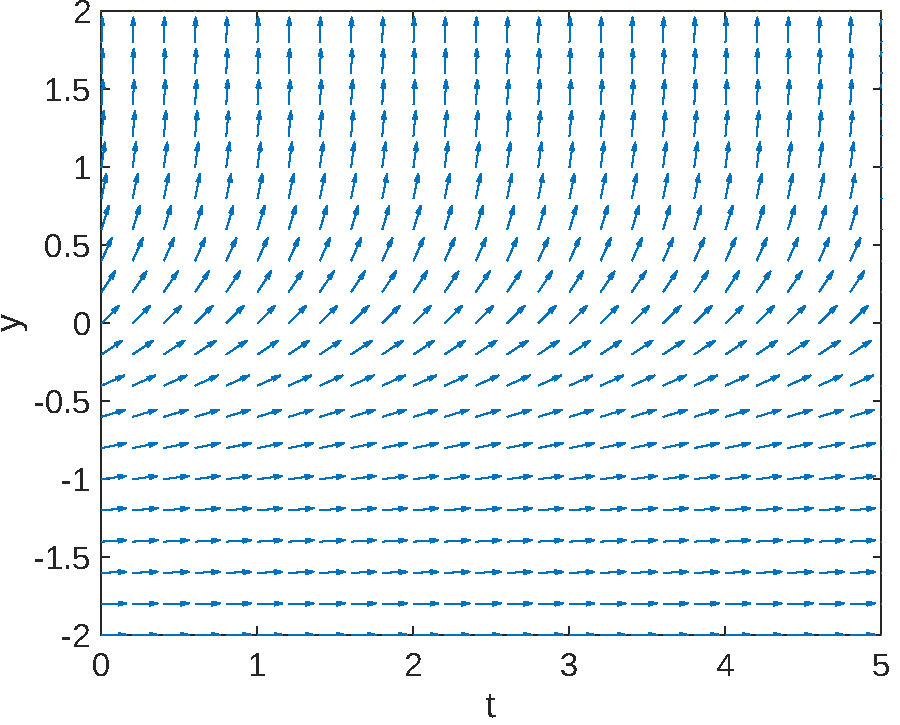
\includegraphics[width=.95\columnwidth]{images/blowup_field.pdf}
}\vfill
Note: The slope is positive for all values of y. Blowup happens for all initial conditions.
\end{frame}



\begin{frame}[fragile]
\vfill
\frametitle{\ex{$y'=\frac{x^2}{y}$}}

\twomini[.7]{.4}{.55}{
\textcolor{black}{
\lstinputlisting[language=Matlab, frame=single]{matlab_scripts/slopefield_ex2.m}
}
}{
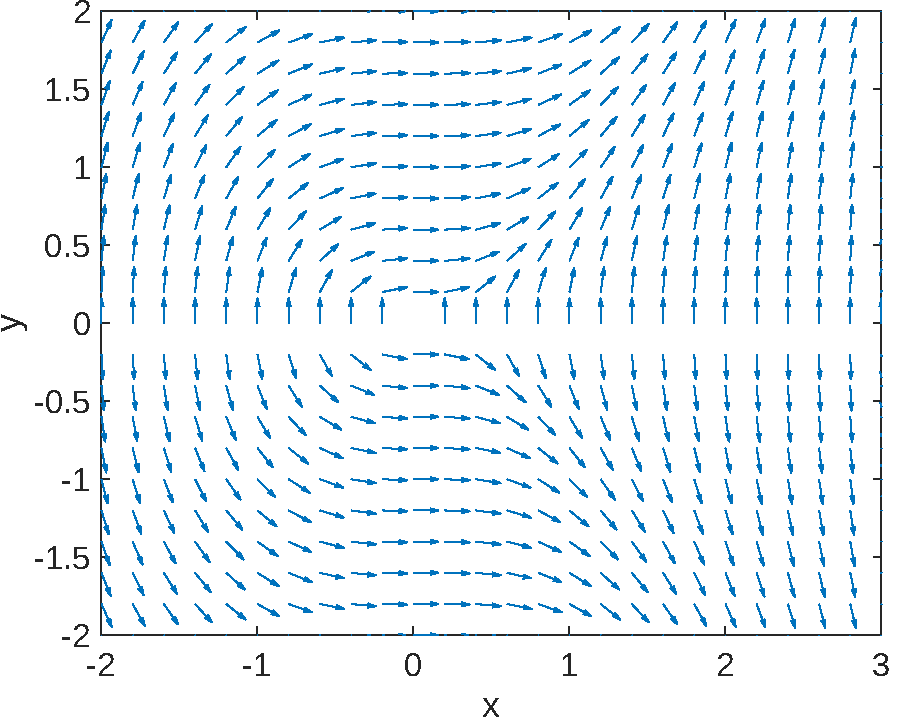
\includegraphics[width=.95\columnwidth]{images/slopefield_ex2.pdf}
}\vfill
Trace a solution backwards from $y(0)=1$.\vfill
Why does the solution not exist for $x<-\sqrt[3]{\nicefrac32}$? \vfill 

\centering \student{$f(x,y)$ is discontinous $y=0$}
\vfill
\end{frame}

\subsection{Existence and uniqueness}

\slide[Picard's Theorem]{
A \uline{unique} solution to
\vfill
 \[y'=f(t,y),\quad \text{with } y(t_0)=y_0\] 
\vfill
exists for t near $t_0$ if\vfill \enum{ \item $f(t,y)$ is continuous (as a function of two variables) and \item $\nicefrac{\partial f}{\partial y}$ exists and is continuous near $(t_0,y_0)$.}

\vfill

}

\slide[\ex{$y'=2\sqrt{|y|}$, with y(0)=0}]{
\twomini[.6]{.6}{.4}{
Analytically, we find 2 solutions
\enum{\item By inspection: \[y(t)=0\] \item Integrate for positive and negative $y$ separately: \[y(t)=\begin{cases}  t^2 & t\geq0 \\ -t^2 & t<0 \end{cases}\] }
}{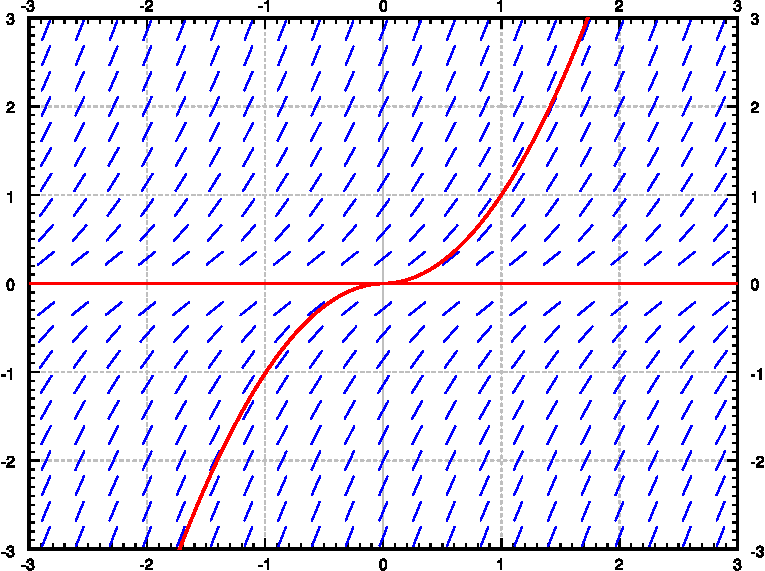
\includegraphics[width=.95\columnwidth]{images/1-3-sqrt-sol-mbx.pdf}}
\vfill
\student{Picard's uniqueness theorem does not apply, because $\pd{}{y}2\sqrt{|y|}$ does not exist at $y=0$.}
}

\end{document}